\chapter{Multi-modal and Multi-scale Time series Metric Learning ({\sc m}$^2${\sc tml}) solution}
\label{chap:implementation}
\minitoc

%\noindent Chapeau introductif :
%\begin{itemize}
%	\item Quel problème on résout?
%	\item Donner les étapes principales de résolution (sous forme de puces). Cela doit rester général, clair et concis.
%	\item Développer dans chaque section les puces énumérés précédemment.
%\end{itemize}

\fbox{  \parbox{0.9\textwidth}{
		In this chapter, we present the steps of our proposed algorithm referred as Multi-modal and Multi-scale Time series Metric Learning ({\sc m}$^2${\sc tml}). \\
		First, we introduce the multi-scale comparison concept for time series. Then, we present the steps to learn a Multi-modal and Multi-scale Time series metric for a robust $k$-Nearest Neighbor classifier: projection in the pairwise space, neighborhood construction and scaling, {\sc svm}-based metric learning resolution, and definition of the dissimilarity measure. We conclude by extending the algorithm {\sc m}$^2${\sc tml} for multivariate and regression problems.
	}  }

%-----------------------------------------------------------------------------
\section{Multi-scale approach}
\label{sec:multiscale}
%\begin{itemize}
%	\item Dans le cadre de la classification, on peut avoir des données où l'information qui permet de discriminer une classe d'une autre n'est pas globale mais est localisé sur une partie du signal
%	\item Limite des métriques basiques présentées précédemment (valeur, forme, fréquence) considère la comparaison sur l'intégralité du signal
%	\item On propose la définition de métriques locales. Pour cela, on va découper notre signal. Il existe plusieurs manières de réaliser ce découpage. On va utiliser la dichotomie proposée par Douzal \& al.
%\end{itemize}

%\noindent Chapeau introductif
%\begin{itemize}
%	\item Objectif : Trouver une distance, combinaison des distances basiques qui donne une bonne classification $k$-NN sur une base de données.
%	\item Pourquoi une distance combinée? Dans le cadre de données réelles, plusieurs modalités peuvent être impliquées (forme, valeur, fréquence), de manière globale ou locale.
%	\item Dans le cadre des données réelles, plusieurs composantes/modalités peuvent être impliqués (forme, valeur, fréquence). = attribut (feature) en traitement du signal. Hypothèse : valeur sur une série complète, sur un intervalle ou sur une fenêtre (dans le cadre des métriques à base fréquentielle).
%\end{itemize}


In some applications, time series may exhibit similarities among the classes based on local patterns in the signal. Fig. \ref{fig:UMD} illustrates a toy example from the {\sc bme} dataset in which time series of different classes seems to be similar on a global scale. However, at a more locally scale, a characteristic upward bell at the beginning or at the end of the time series allows to differentiate the class B (upward bell at the beginning) from the class E (upward bell at the end). Also, in massive time series datasets, computing the metric on all time series elements $x_{it}$ might become time consuming. Computing the metric on a smaller part of the signal and not all the time series elements $x_{it}$ makes the metric computation faster.

\begin{figure}[h!]
	\centering
	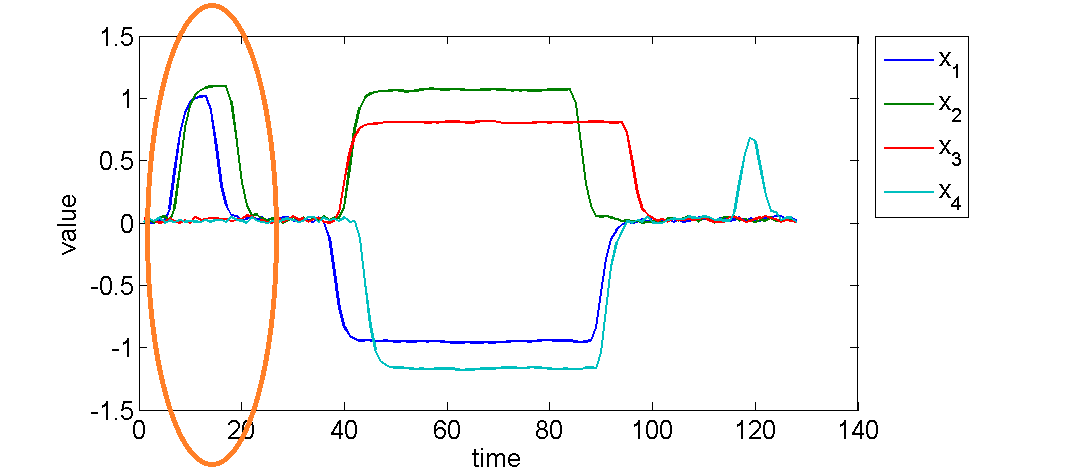
\includegraphics[width=0.8\linewidth]{images/BME_local}
	\caption{Example of 4 time series from the BME dataset, made of 3 classes : Begin, Middle and End. The 'Up' class has a characteristic bell at the beginning of the time series. The 'End' class has a characteristic bell at the end of the time series. The 'Middle' class has no characteristic bell. Orange circle show the region of interest of these bells for the class 'Begin'. This region is local and standard global metric fails to show these characteristics.}
	\label{fig:UMD}
\end{figure}

Localizing patterns of interest in huge time series datasets has become an active area of search in many applications including diagnosis and monitoring of complex systems, biomedical data analysis, and data analysis in scientific and business time series \todo{ref}. A large number of methods have been proposed covering the extraction of local features from temporal windows \cite{Berndt1994a} or the matching of queries according to a reference sequence \cite{Faloutsos1994}. We focus on the computation of "local metrics".

It can be noted that the distance measures (amplitude-based $d_A$\footnote{We recall that $d_A$ is the Euclidean distance $d_E$ in our work.}, frequential-based $d_F$, behavior-based $d_B$) in Eqs. \ref{eq:A}, \ref{eq:F} and \ref{eq:B} implies systematically the total time series elements $x_{it}$ and thus, restricts the distance measures to capture local temporal differences. In our work, we provide a multi-scale framework for time series comparison using a hierarchical structure. Many methods exist in the literature such as the sliding window or the dichotomy \todo{ref}. We detailed here the latter one.


A multi-scale description can be obtained by repeatedly segmenting a time series expressed at a given temporal scale to induce its description at a more locally level. Many approaches have been proposed assuming fixed either the number of the segments or their lengths. In our work, we consider a binary segmentation at each level. Let $I=[a;b]$ be a temporal interval of size $(b-a)$. The interval $I$ is decomposed into two equal overlaped intervals $I_L$ (left interval) and $I_R$ (right interval). A parameter $\alpha$ that allows to overlap the two intervals $I_L$ and $I_R$, covering discriminating subsequences in the central region of $I$ (around $\frac{b-a}{2}$):
% For a strict division (no overlapping), the dichotomy process divide $I$  into two equal intervals at $\frac{b-a}{2}$: the left one $I_L$ and the right $I_R$ one. We add a parameter $\alpha$ that allows to overlap the two intervals $I_L$ and $I_R$, covering discriminating subsequences in the central region of I (around $\frac{b-a}{2}$) and thus avoiding 'border effects':
\begin{align}
	I &= [a;b] \\
	I_L &= [a;a+\alpha(b-a)] \\
	I_R &= [a-\alpha(b-a);b] 
	\label{key}
\end{align}

\noindent For $\alpha = 0.6$, the overlap covers $10\%$ of the size of the interval $I$. Then, the process is repeated on the intervals $I_L$ and $I_R$. We obtain a set of intervals $I_s$ illustrated in Fig. \ref{fig:Intervalles}.

\begin{figure}[h!]
	\centering
	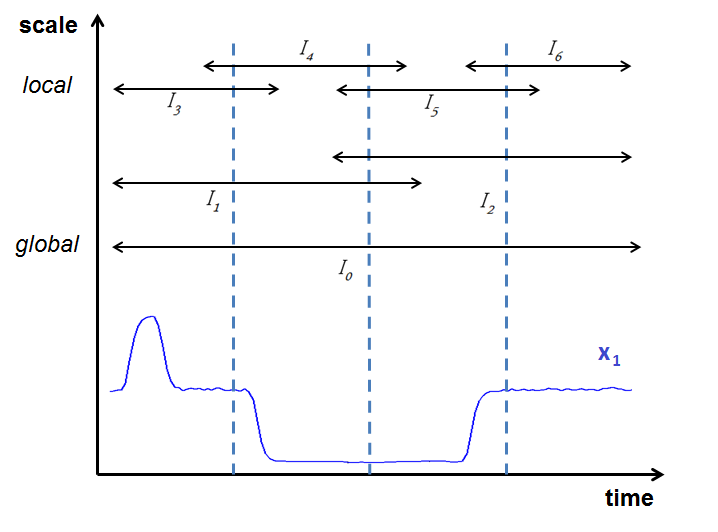
\includegraphics[width=0.7\linewidth]{images/Intervalles3}
	\caption{Multi-scale decomposition}
	\label{fig:Intervalles}
\end{figure}

\noindent A multi-scale description is obtained on computing the usual time series metrics ($d_A$, $d_B$, $d_F$) on the resulting segments $I_s$. Note that for two time series $\textbf{x}_i$ and $\textbf{x}_j$, the comparison between $\textbf{x}_i$ and $\textbf{x}_j$ is done on the same interval $I_s$. For a multi-scale amplitude-based comparison based on binary segmentation, the set of involved amplitude-based measures $d^{Is}_A$ is:
\begin{equation}	
d^{Is}_A(\textbf{x}_i,\textbf{x}_j) = \sqrt{\sum\limits_{t \in Is} (x_{it}-x_{jt})^2}
\label{eq:A2}
\end{equation}
The local behaviors- and frequential- based measures $d^{Is}_B$ and $d^{Is}_F$ are obtained similarly.



%---------------------------------------------------------------------------
\section{Projection in the dissimilarity space}
%\begin{itemize}
%	\item Projection
%	\item Log normalization
%\end{itemize}
Let $\{\textbf{x}_i; y_i\}_{i=1}^n$ be $n$ time series $\textbf{x}_i \in \mathbb{R}^Q$ of length $Q$ and of class label $y_i$. Let $d_1, \ldots, d_p$ be the set of multi-modal and multi-scale dissimilarity measures $d_A^{I_s}$, $d_B^{I_s}$ and $d_F^{I_s}$ related to segments $I_s$ of
several temporal scales, as described in Section \ref{sec:multiscale}.

\noindent \textbf{Projection in the pairwise space} \\
We note $\psi$ an embedding function that maps each pair of time
series $(\textbf{x}_i; \textbf{x}_j)$ to a vector $\textbf{x}_{ij}$ in a dissimilarity space $\mathbb{R}^p$ whose dimensions are the dissimilarities $d_1, \ldots, d_p$ as explained in Chapter \ref{sec:TML}:
\begin{equation}
	\begin{aligned}
	\psi : \mathbb{R}^Q \times \mathbb{R}^Q & \rightarrow \mathcal{E} \\
	(\textbf{x}_i; \textbf{x}_j) & \rightarrow \textbf{x}_{ij} = [d_1(\textbf{x}_i; \textbf{x}_j), \ldots, d_p(\textbf{x}_i; \textbf{x}_j)]^T
	\end{aligned}
	\label{eq:projection}
\end{equation}

We cast the problem of learning a multi-modal and multiscale temporal metric as learning the metric $D$ a combination function of $d_1, \ldots, d_p$ in the pairwise space $\mathcal{E}$:
\begin{equation}
D = f(d_1, \ldots , d_p)
\end{equation}
The learning process is guided by local constraints to ensure dissimilarities between neighbors of a same class (i.e. $y_{ij}=-1$) lower than the dissimilarity between neighbors of different classes ($y_{ij}=+1$). The learned metric $D$ should satisfy, in addition, the properties of a dissimilarity measure, i.e. positivity ($D(\textbf{x}_{ij}) \geq 0$), distinguishability ($D(\textbf{x}_{ij}) = 0 , \textbf{x}_i = \textbf{x}_j$) and symmetry ($D(\textbf{x}_{ij}) = D(\textbf{x}_{ji})$). \\



\noindent \textbf{Pairwise space normalization} \\
The scale between the $p$ basic metrics $d_h$ can be different. Thus, there is a need to scale the data within the pairwise space and ensure comparable ranges for the $p$ basic metrics $d_h$. In our experiment, we use dissimilarity measures with values in $[0;+\infty[$. Therefore, we propose to Z-normalize their log distributions as explained in Section \ref{sec:data_normalization}. \\

% \todo{A simplifier d'après Michèle}
% In the following we detail the two main steps of the proposed solution {\sc m}$^2${\sc tml}. First, the neighborhood for each time series $\textbf{x}_i$ is built to construct the pairwise training set $\{\textbf{x}_{ij},y_{ij}\}$. Secondly, an {\sc svm} is operated in the pairwise space $\mathcal{E} = \bigcup\limits_{i} \{\textbf{x}_{ij},y_{ij}\}$ to learn a direction (i.e. weights) that discriminates positive ($y_{ij}=+1$) from negative ($y_{ij}=-1$) pairs. Thirdly, an exponential transformation of the projected norm on the learned discriminative direction allows to induce a dissimilarity measure that satisfy all required conditions, as well as homogeneous neighborhoods for a robust $k$-NN classification.

%---------------------------------------------------------------------------
\section{Neighborhood construction and scaling}
\label{sec:neighborhood}
%\begin{itemize}
%	\item Expliquer les différentes stratégies (k-NN VS All / M-NN VS M-diff / k-NN VS Imposters)
%	\item Expliquer pourquoi on va choisir une stratégie M-NN VS M-diff
%\end{itemize}
The metric learning problem aims to learn a metric $D$ that pulls the $k$ nearest neighbors (targets) while pushing the time series of different classes. Thus, the preliminary step defines the target pairs. For that, an initial distance is necessary to build the neighborhood. 

Let $\textbf{x}_{ij} \in \mathbb{R}^p$ $i,j \in \{1,\ldots,n\}$ be a set of samples into the pairwise space $\mathcal{E}$ as described in Eq. \ref{eq:projection}. For each time series $\textbf{x}_{i}$, we denote $X_i^+$ the set of \textbf{positive pairs} $\textbf{x}_{ij}$ such that $y_{ij}=+1$ (i.e. the time series $\textbf{x}_i$ and $\textbf{x}_j$ has different class label $y_j \neq y_i$). Similarly, we denote $X_i^-$ the set of \textbf{negative pairs} $\textbf{x}_{ij}$ such that $y_{ij}=-1$ (i.e. the time series $\textbf{x}_i$ and $\textbf{x}_j$ has the same class label $y_j = y_i$):
\begin{align}
	X_i^- = \{\textbf{x}_{ij},y_{ij}=-1\} &\text{\quad (same class)} \\
	X_i^+ = \{\textbf{x}_{ij},y_{ij}=+1\} &\text{\quad (different classes)}
\end{align}
As the learned distance $D$ is not known, without prior knowledge, we choose a $L_2$ norm as an initial metric to define the positive and negative sets:\\
\begin{equation}
||\textbf{x}_{ij}||_2 = \sqrt{\sum\limits_{h=1}^{p}\left( d_h(\textbf{x}_{i}, \textbf{x}_{j})\right)^2}
\end{equation}
The \textbf{target set} $X_i^{-*}$ is a subset of the negative set $X_i^-$ of pairs $\textbf{x}_{ij}$ such that the time series $\textbf{x}_{j}$ are the $k$-nearest neighbors of $\textbf{x}_{i}$, denoted $j \rightsquigarrow i$:
\begin{align}
X_i^{-*} = \{\textbf{x}_{ij},y_{ij}=-1\} &\text{\quad s.t.   } j \rightsquigarrow i
\end{align}
The $k$ nearest neighbors of a sample $\textbf{x}_i$, denoted $\textbf{x}_j$ ($j \rightsquigarrow i$),  are defined in the pairwise space $\mathcal{E}$ by the $k$-th lowest norm $||\textbf{x}_{ij}||_2$ negative pairs. Similarly, the \textbf{imposter set} $X_i^{+*}$ is a subset of the positive set $X_i^+$ of pairs $\textbf{x}_{il}$ such that the time series $\textbf{x}_{l}$ is an imposter of $\textbf{x}_{i}$, denoted $l \nrightarrow i$. It corresponds the pairs $\textbf{x}_{il}$ that have a $L_2$ norm lower that the $L_2$ norm of the $k$-th nearest neighbor:
\begin{align}
X_i^{+*} = \{\textbf{x}_{il},y_{il}=+1\} &\text{\quad s.t.   } l \nrightarrow i
\end{align}
\noindent To build the pairwise training set $X_p$, three solutions are proposed, illustrated in Fig \ref{fig:Strategy_neighborhood}: 
\begin{enumerate}
	\item \textbf{$k$-NN vs impostors}: it corresponds to the union for all $\textbf{x}_i$ of the target set and impostor set:
		\begin{equation}
			X_p = \bigcup\limits_{i} \left( X_i^{-*} \cup X_i^{+*} \right) 
		\end{equation}
	\item \textbf{$k$-NN vs all}: it corresponds to the union for all $\textbf{x}_i$ of the target set and positive set. It ensures that no pairs $\textbf{x}_{il}$ of different classes will invade the target neighborhood during the learning process:
		\begin{equation}
			X_p = \bigcup\limits_{i} \left( X_i^{-*} \cup X_i^{+} \right) 
		\end{equation}
	
	\item \textbf{$m$-NN$^+$ vs $m$-NN$^-$}: it corresponds to the union for all $\textbf{x}_i$ of the set of the $m$-nearest neighbors of the same class, denoted $m$-NN$^-_i$, and the $m$-nearest neighbor of $\textbf{x}_i$ of a different class ($y_j \neq y_i$), denoted $m$-NN$^+_i$. For a $k$-NN classifier, by considering larger neighborhoods with $m=\alpha k(\alpha>1)$ one includes more variability to generalize better the obtained solution:
		\begin{equation}
			X_p = \bigcup\limits_{i} \left( m\text{-NN}^+_i \cup m\text{-NN}^-_i \right) 
		\end{equation}
	In the following, for simplification purpose, we define $m\text{-NN}^- = \bigcup\limits_{i} m\text{-NN}^-_i$ as the union of all of the set of the $m$-nearest neighbors of the same class and $m\text{-NN}^- = \bigcup\limits_{i} m\text{-NN}^+_i$ as the $m$-nearest neighbor of $\textbf{x}_i$ of a different class.
\end{enumerate}
\begin{figure}[h!]
\centering
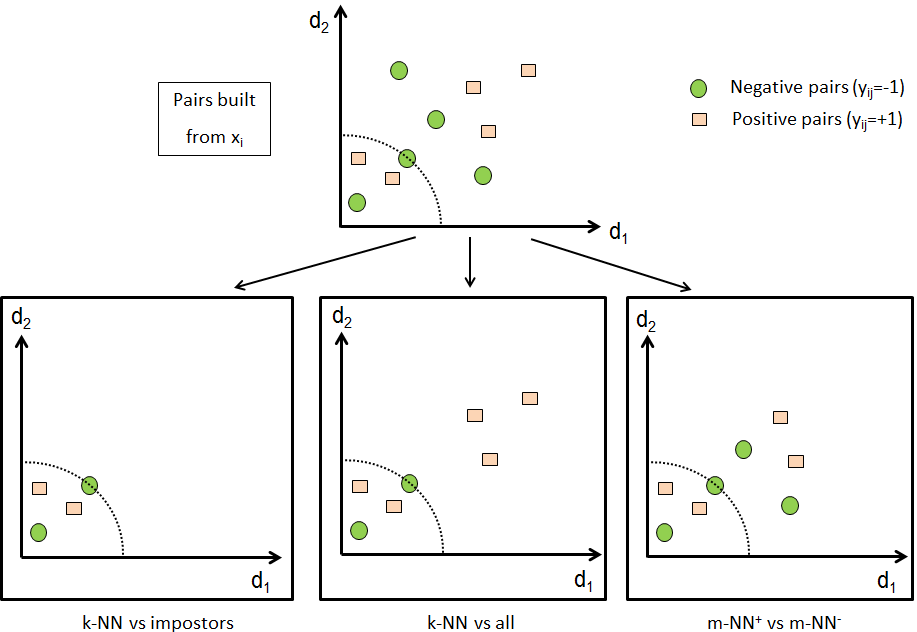
\includegraphics[width=0.95\linewidth]{images/Strategy_neighborhood}
\caption{Example of a $k$-NN problem with $k=2$. 3 different strategies (bottom) for pairwise training set $X_p$ construction from the embedding of time series $\textbf{x}_i$ in the pairwise space (top): $k$-NN vs impostor strategy (left), $k$-NN vs all strategy (middle) and $m$-NN$^+$ vs $m$-NN$^-$ (right) with $m=4$.}
\label{fig:Strategy_neighborhood}
\end{figure}
In our experiment, we use the $m$-NN$^+$ vs $m$-NN$^-$ strategy for better generalization of the solution compared to $k$-NN vs impostors strategy and for faster solutions compared to $k$-NN vs all strategy. Note that in $m$-NN$^+$ vs $m$-NN$^-$ strategy, the set of positive and negative pairs is balanced.


%---------------------------------------------------------------------------
%%\section{Neighborhood scaling}
%\begin{itemize}
%	\item Expliquer le problème de la non-homogénéité des radius.
%	\item Expliquer comment on résout ce problème par une normalisation des radius de chaque voisinage.
%\end{itemize}
\noindent \textbf{Neighborhood scaling} \\
Let $r_i$ be the radius associated to $\textbf{x}_i$ corresponding to the maximum norm of its $m$-th nearest neighbor of same class in $m$-NN$^-$:
\begin{equation}
	r_i = \max_{\textbf{x}_{ij} \in \text{$m$-NN$^-$}} ||\textbf{x}_{ij}||_2
\end{equation}
As explained in Chapter \ref{sec:TML}, Section \ref{sec:relationship}, there exists an heterogeneity in the neighborhood. In real datasets, local neighborhoods can have very different scales as illustrated in Fig. \ref{fig:Neighborhood_scaling_problem}. To make the target neighborhood spreads comparable, we propose for each $\textbf{x}_i$ to scale its neighborhood vectors $\textbf{x}_{ij}$ such that the $L_2$ norm (radius) of the farthest $m$-th nearest neighbor is 1:
\begin{equation}
	\textbf{x}_{ij}^{norm} = \left[ \frac{d_1(\textbf{x}_{ij})}{r_i}, \ldots, \frac{d_p(\textbf{x}_{ij})}{r_i}\right] ^T
\end{equation}
For simplification purpose, we denote in the following $\textbf{x}_{ij}$ as $\textbf{x}_{ij}^{norm}$. Fig. \ref{fig:Neighborhood_scaling} illustrates the effect of neighborhood scaling in the pairwise space.
\begin{figure}[h!]
	\centering
	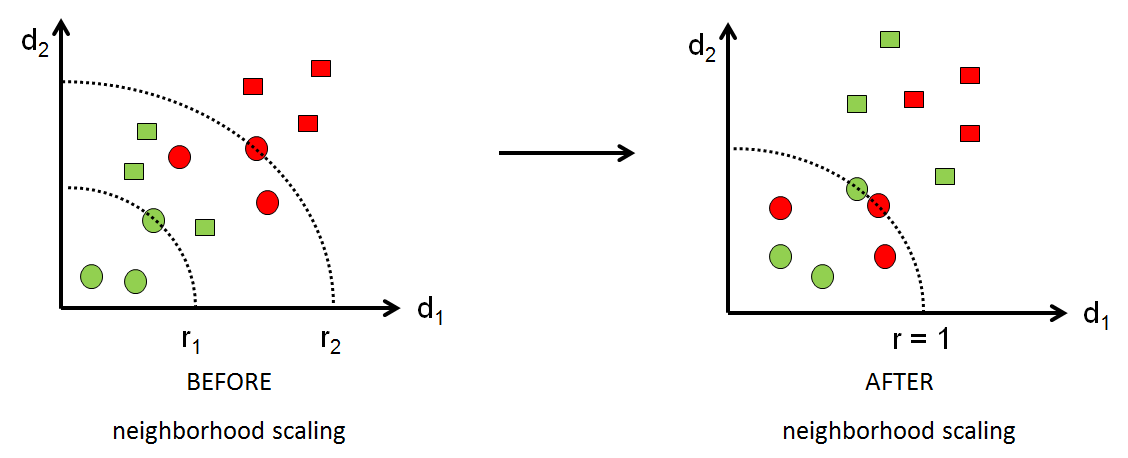
\includegraphics[width=1\linewidth]{images/Neighborhood_scaling}
	\caption{Effect of neighborhood scaling before (left) and after (right) on the neighborhood of two time series $\textbf{x}_1$ (green) and $\textbf{x}_2$ (red). Circle represent negative pairs ($m\text{-NN}^-$) and square represents positive pairs ($m\text{-NN}^+$) for $m=2$ neighbors. Before scaling, the problem is not linearly separable. The spread of each neighborhood are not comparable. After scaling, the target neighborhood becomes comparable and in this example, the problem becomes linearly separable between the circles and the squares.}
	\label{fig:Neighborhood_scaling}
\end{figure}
%---------------------------------------------------------------------------
%---------------------------------------------------------------------------
\section{Definition of the dissimilarity measure}
\subsection{Support Vector Machine ({\sc svm}) resolution}
% \section{Solving the Support Vector Machine ({\sc svm}) problem}
%\begin{itemize}
%	\item Expliquer l'apprentissage avec le SVM.
%	\item Utilisation de la version L1 du SVM pour avoir une solution sparse.
%\end{itemize}
Let $\{\textbf{x}_{ij}; y_{ij} = \pm 1\}$, $\textbf{x}_{ij} \in m\text{-NN}^+ \cup \text{  } m\text{-NN}^-$ be the training set, with $y_{ij} = +1$ for $\textbf{x}_{ij} \in$ $m$-NN$^+$ (same label) and $-1$ for $\textbf{x}_{ij} \in$ $m$-NN$^-$ (different labels). For a maximum margin between positive and negative pairs, the problem is formalized in an {\sc svm} framework as follows in the pairwise space $\mathcal{E}$:
\begin{align}
	& \argmin_{\textbf{w},b,\boldsymbol{\xi}} \frac{1}{2}||\textbf{w}||_2^2 + C \sum\limits_{i,j} \xi_{ij} \label{eq:svm_pairwise}\\
	&\textbf{s.t. } y_{ij}(\textbf{w}^T \textbf{x}_{ij} + b) \geq 1-\xi_{ij} \\
	&\xi_{ij} \geq 0
\end{align}
Thanks to the unit radii normalization $\textbf{x}_{ij}/r_i$, the {\sc svm} ensures a global large margin solution involving equally local neighborhood constraints (i.e. local margins). \\
In the linear case, a $L_1$ regularization in Eq. \ref{eq:svm_pairwise} leads to a sparse and interpretable \textbf{w} that uncovers the modalities, periods and scales that differentiate best positive from negative pairs for a robust nearest neighbors classification:
\begin{align}
& \argmin_{\textbf{w},b,\boldsymbol{\xi}} ||\textbf{w}||_1 + C \sum\limits_{i,j} \xi_{ij} \label{eq:svm_pairwiseL1}
\end{align}

%\begin{itemize}
%	\item Produit scalaire
%	\item Papier PR : norme pondérée x fonction exponentielle
%	\item Version Sylvain : norme x fonction exponentielle?
%\end{itemize}
The proposed {\sc m}$^2${\sc tml} approach differs from the one of Time series Metric Learning ({\sc tml}) by Linear/Quadratic programming ({\sc lp}/{\sc qp}) in which a {\sc svm} pairwise is used to learn the best weight vector $\textbf{w}$ such that positive pairs are widely separated from negative pairs. Defining the learned metric $D$ from the vector $\textbf{w}$ needs to be careful.

\subsection{Linear solutions}
Let $\textbf{x}_{test}$ be a new sample, $\textbf{x}_{i,test} \in \mathcal{E}$ gives the proximity between $\textbf{x}_{i}$ and $\textbf{x}_{test}$ based on the $p$ multi-modal and multi-scale metrics $d_h$. We denote $\textbf{P}_\textbf{w}(\textbf{x}_{i,test})$ the orthogonal projection of $\textbf{x}_{i,test}$ on the axis of direction \textbf{w} and $||\textbf{P}_\textbf{w}(\textbf{x}_{i,test})||$ its norm that allows to measure the closeness between $\textbf{x}_{test}$ and $\textbf{x}_{i}$ while considering the discriminative features between positive and negative pairs. We review in this section different propositions to define the learned metric $D$: Scalar product, Projection Norm, Exponential transformation. \\

\noindent \textbf{Problem linked to the {\sc svm} resolution} \\
First, the learned metric $D$ can be defined as the decision function obtained by solving the {\sc svm} problem:
\begin{equation}
D(\textbf{x}_{i,test}) = \textbf{w}^T\textbf{x}_{i,test} + b
\end{equation}
The obtained metric $D$ doesn't necessarily satisfy the distinguishability ($D(\textbf{x}_{ii}=0)$) and positivity ($D(\textbf{x}_{ij} \geq 0)$) property, especially when positive pairs (different classes) are situated nearer to the origin point than negative pairs (same class) (Fig. \ref{fig:Dissimilarity_def_scalar_product}).
\begin{figure}[h!]
\centering
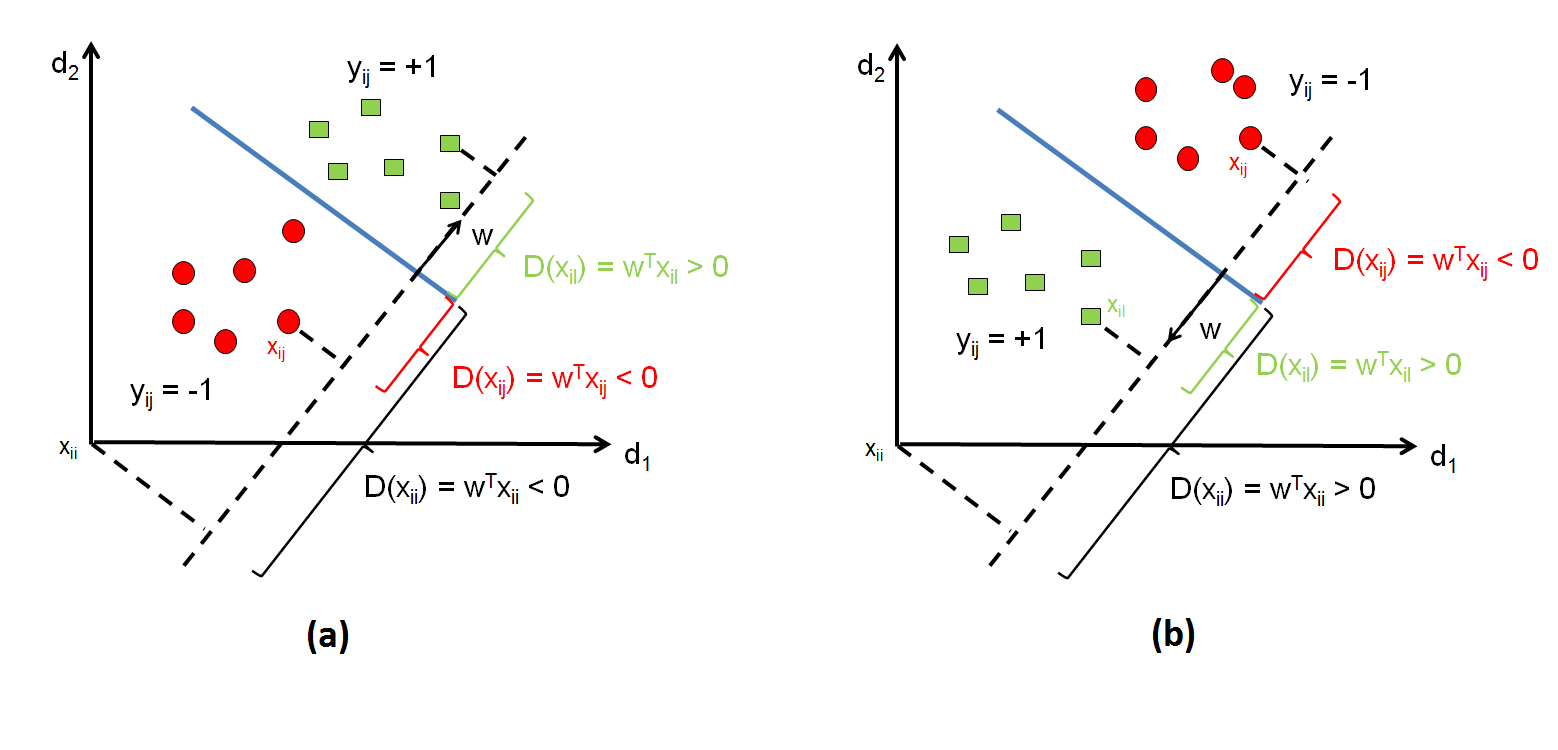
\includegraphics[width=1\linewidth]{images/Dissimilarity_def_scalar_product}
\caption{Example of {\sc svm} solutions and of the resulting metric $D$ defined by a scalar product. Fig. (a) represents common expected configuration where negative pairs ($\textbf{x}_i$ and $\textbf{x}_j$ are of same class) are situated in the same side as the origin $\textbf{x}_{ii}=0$. In Fig. (b), the vector $\textbf{w}=[-1 -1]$ indicates that positive pairs ($y_{ij}$) are on the side of the origin point. For the two configurations, two problems arises: First, for negative pairs, $D(\textbf{x}_{ij}) \leq 0$. Secondly, for the origin point $\textbf{x}_{ii}$, we obtain $D(\textbf{x}_{ii}) \neq 0$.}
\label{fig:Dissimilarity_def_scalar_product}
\end{figure}


\noindent The norm of the projection $\textbf{P}_\textbf{w}(\textbf{x}_{i,test})$ can be used to define the learned metric $D$ as it measures the distance of the pair $\textbf{x}_{i,test}$ from the origin point $\textbf{x}_{ii}$ along to the direction $\textbf{w}$:
\begin{equation}
	D(\textbf{x}_{i,test}) = ||\textbf{P}_\textbf{w}(\textbf{x}_{i,test})|| = ||\textbf{w}^T\textbf{x}_{i,test}||
\end{equation}
Although the norm $||\textbf{P}_\textbf{w}(\textbf{x}_{i,test})||$ satisfies metric properties, it doesn’t always guarantee lower distances between negative pairs (same class) than positive pairs (different classes) as illustrated in Fig \ref{fig:Dissimilarity_def_norm_scalar_product}. 

\begin{figure}[h!]
	\centering
	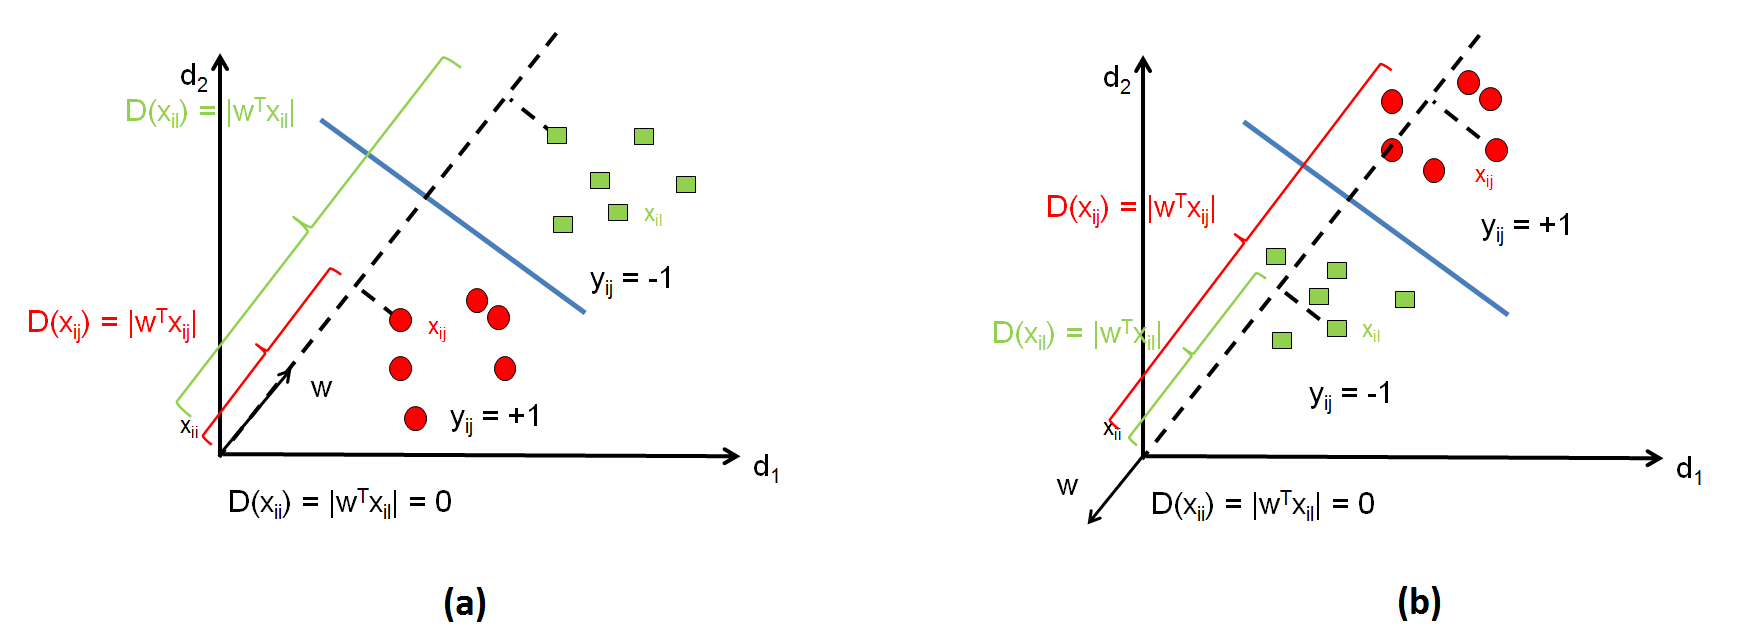
\includegraphics[width=1\linewidth]{images/Dissimilarity_def_norm_scalar_product}
	\caption{Example of {\sc svm} solutions and of the resulting metric $D$ defined by the norm of the projection on $\textbf{w}$. Fig. (a) represents common expected configuration where negative pairs ($\textbf{x}_i$ and $\textbf{x}_j$ are of same class) are situated in the same side as the origin $\textbf{x}_{ii}=0$. In Fig. (b), the vector $\textbf{w}=[-1 -1]$ indicates that positive pairs ($y_{ij}$) are on the side of the origin point. One problem arrises in Fig. (b): distance of positive pairs $D(\textbf{x}_{il})$ is lower than the distance of negative pairs $D(\textbf{x}_{ij})$.}
	\label{fig:Dissimilarity_def_norm_scalar_product}
\end{figure}


\noindent \textbf{Exponential transformation} \\
Secondly, we propose to add an exponential term to operate a "push" on negative pairs based on their distances to the separator hyperplan, that leads to the dissimilarity measure $D$ of required properties:
\begin{equation}
	D(\textbf{x}_{i,test}) = 
	||\textbf{P}_\textbf{w}(\textbf{x}_{i,test})||.
	\exp(\lambda[\textbf{w}\textbf{P}_\textbf{w}(\textbf{x}_{i,test}) + b]_+)
	 \text{ \quad  } \lambda > 0
	\label{eq:dissimilarity_learn}
\end{equation}
where $\lambda$ controls the "push" term and $\textbf{w}\textbf{P}_\textbf{w}(\textbf{x}_{i,test}) + b$ defines the distance between the orthogonal projected vector and the separator hyperplane; $[t]_+ = \max(0; t)$ being the positive operator. Note that, for a pair lying into the negative side ($y_{ij} = -1$), $[\textbf{w}\textbf{P}_\textbf{w}(\textbf{x}_{i,test}) + b]_+ = 0$, the exponential term is vanished (i.e. no "pull" action) and the dissimilarity leads to the norm term. For a pair situated in the positive side ($y_{ij} = +1$), the norm is expanded by the push term, all the more the distance to the hyperplane is high.

\begin{figure}[h!]
	\centering
	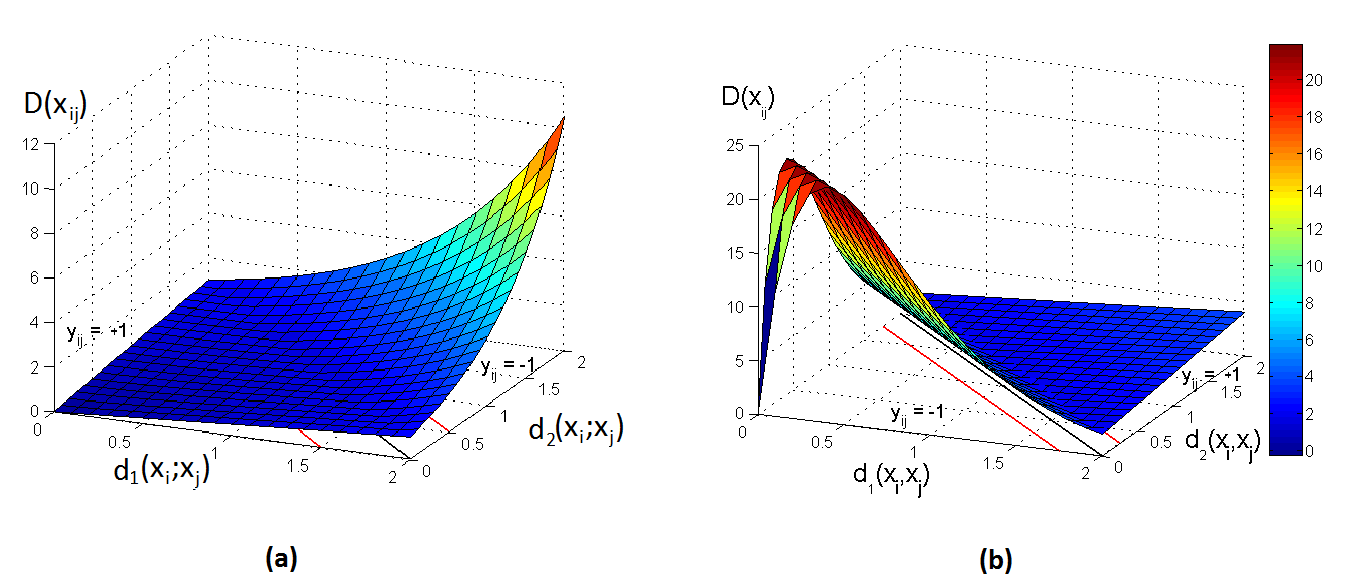
\includegraphics[width=1\linewidth]{images/3D_diss}
	\caption{The behavior of the learned metric $D$ ($p = 2$; $\lambda = 2.5$) with respect to common (a) and challenging (b) configurations of positive and negatives pairs.}
	\label{fig:3D_diss}
\end{figure}

%\begin{figure}[h!]
%	\centering
%	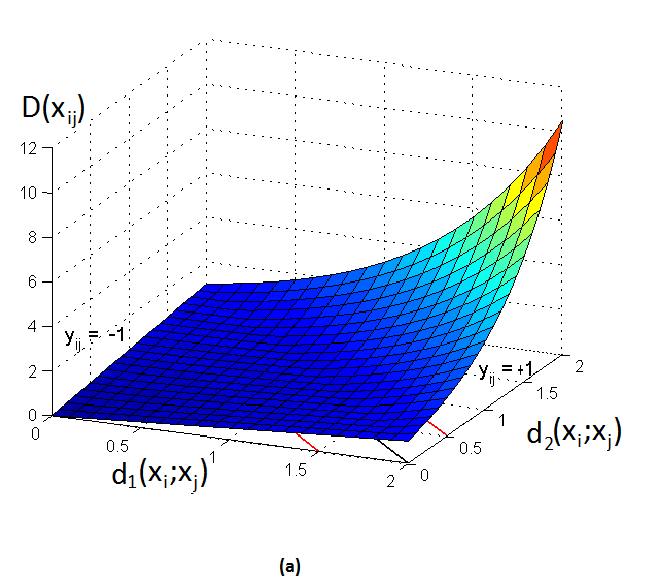
\includegraphics[width=0.6\linewidth]{images/3D_positive1}
%	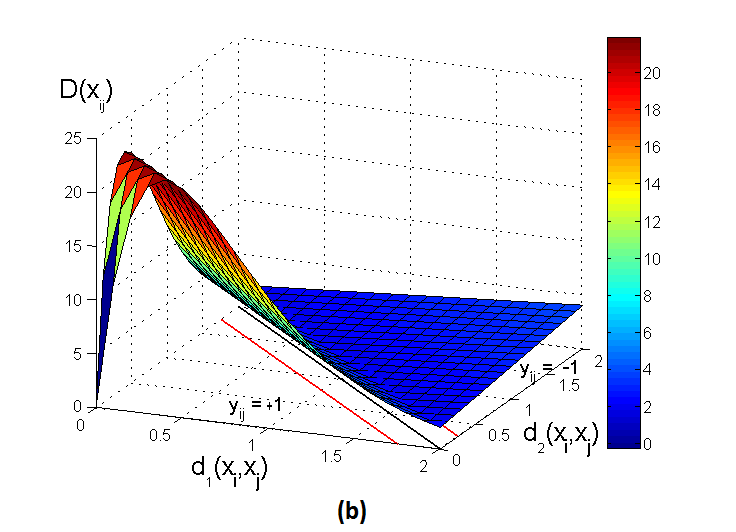
\includegraphics[width=0.6\linewidth]{images/3D_negative}
%	\caption{The behavior of the learned metric $D$ ($p = 2$; $\lambda = 2.5$) with respect to common (a) and challenging (b) configurations of positive and negatives pairs.}
%	\label{fig:3D_diss}
%\end{figure}

Fig. \ref{fig:3D_diss}, illustrates for $p = 2$ the behavior of the learned dissimilarity according to two extreme cases. The first one (Fig. \ref{fig:3D_diss}-a), represents common expected configuration where negative pairs ($\textbf{x}_i$ and $\textbf{x}_j$ are of same class) are situated in the same side as the origin. The dissimilarity increases proportionally to the norm in the negative side, then exponentially on the positive side. Although the expansion operated in the positive side is dispensable in that case, it doesn’t affect nearest neighbors classification. Fig. \ref{fig:3D_diss}-b, shows a challenging configuration where positive pairs ($\textbf{x}_i$ and $\textbf{x}_j$ are of different classes) are situated in the same side as the origin. That means that time series $\textbf{x}_j$ that are of different classes from $\textbf{x}_i$ are closer to $\textbf{x}_i$ than its nearest neighbors. They are thus impostors. The dissimilarity behaves proportionally to the norm on the negative side, and increases exponentially from the hyperplane until an abrupt decrease induced by a norm near 0. Note that the region under the abrupt decrease mainly uncovers false positive pairs, i.e., pairs of norm zero labeled differently.

\subsection{Non-linear solutions}
The above solution holds true for any kernel $K$ and allows to extend the dissimilarity $D$ given in Eq. \ref{eq:dissimilarity_learn} to non linearly separable positive and negative pairs. Let $K$ be a kernel defined in the pairwise space $\mathcal{E}$ and the related Hilbert space (feature space) $\mathcal{H}$. For a non linear combination function of the metrics $d_h, h = 1,\ldots,p$ in $\mathcal{E}$, we define the dissimilarity measure $D_\mathcal{H}$ in the feature space $\mathcal{H}$ as:

\begin{equation}
\begin{aligned}
	D_\mathcal{H}(\textbf{x}_{i,test}) = 
	& (||\textbf{P}_\textbf{w}(\phi(\textbf{x}_{i,test}))||-||\textbf{P}_\textbf{w}(\phi(\textbf{0}))||). \\
	& \exp\left( \lambda \left[  \sum_{ij}y_{ij} \alpha_{ij} K(\textbf{x}_{ij},\textbf{x}_{i,test}) + b \right] _+\right) 
	\text{ \quad  } \lambda > 0
	\label{eq:dissimilarity_learn_NonLinear}
\end{aligned}
\end{equation}

\noindent with $\phi(\textbf{w})$ the image of \textbf{w} into the feature space $\mathcal{H}$ and the norm of the orthogonal projection of $\phi(\textbf{x}_{i,test})$ on $\phi(\textbf{w})$ as:

\begin{equation}
||\textbf{P}_\textbf{w}(\textbf{x}_{i,test})|| = \frac
	{\sum_{ij} y_{ij} \alpha_{ij} K(\textbf{x}_{ij},\textbf{x}_{i,test})}
	{\sqrt{\sum_{ijkl} \alpha_{ij} \alpha_{kl} y_{ij} y_{kl}
		K(\textbf{x}_{ij},\textbf{x}_{kl})
	}}
\end{equation}
Note that as $\phi(\textbf{0})$ doesn’t meet the origin in the feature space $\mathcal{H}$, the norms in Eq. \ref{eq:dissimilarity_learn_NonLinear} are centered with respect to $\phi(\textbf{0})$. 

We note that the proposed learned metric $D$ and $D_\mathcal{H}$ are heuristic that solves the problem of positive pairs $\textbf{x}_{il}$ on the side of the origin point $\textbf{x}_{ii}$. Other solutions could have been proposed. In practice, the proposed $D$ and $D_\mathcal{H}$ provides suitable solutions for our datasets.
%\noindent \textbf{Limitations} \\
% \todo[inline]{A voir si je complète avec les figures de Sylvain} 



%---------------------------------------------------------------------------
\section{Algorithms and extensions}
\subsection{Algorithms}
\noindent Algorithm 1 summarizes the main steps to learn a multi-modal and multi-scale metric $D$ for a robust nearest neighbors classification. Algorithm 2 details the steps to classify a new sample $\textbf{x}_{test}$ using the learned metric $D$. \todo{Note sur le neighborhood scaling en test?}

\begin{algorithm}[h!]
	\begin{algorithmic}[1]
		\caption{Multi-modal and Multi-scale Temporal Metric Learning ({\sc m}$^2${\sc tml}) for $k$-NN classification}
		\label{algo:MMTML}
		\STATE Input:  
		$X=\{\textbf{x}_i, y_i\}_{i=1}^N$ $N$ labeled time series \\ \hspace{1.1cm} $d_1, ...,d_p$  metrics as described in Eqs. \ref{eq:A}, \ref{eq:F}, \ref{eq:B}, \ref{eq:A2} \\
		\hspace{1.1cm} a kernel $K$
		\STATE Output:  the learned dissimilarity $D$ or $D_{\mathcal{H}}$ depending of $K$ \\
		\STATE  {\it Pairwise embedding} \\   
		Embed pairs $(\textbf{x}_i,\textbf{x}_j)$ $i,j \in {1,...,N}$ into $\mathcal{E}$ as described in Eq. \ref{eq:projection} and normalize $d_h$s
		\STATE  {\it Build positive and negative pairs} \\   
		Build the sets of positive $m$-NN$^+$ and negative $m$-NN$^-$ pairs and scale the radii to 1 as described in \ref{sec:neighborhood}
		% \STATE Define the training set $\{\textbf{x}_{ij}, y_{ij}= \pm 1\}$ with  $\textbf{x}_{ij} \in m$NN+ $\cup$ $m$NN- 
		\STATE Train a {\sc svm}  for a large margin classifier between  $m$-NN$^+$  and $m$-NN$^-$ (Eq. \ref{eq:svm_pairwise})
		\STATE {\it Dissimilarity definition} \\ 
		Consider Eq. \ref{eq:dissimilarity_learn} (resp. Eq. \ref{eq:dissimilarity_learn_NonLinear}) to define $D$ (resp. $D_{\mathcal{H}}$) a linear (resp. non linear) combination function of the metrics $d_h$s.
	\end{algorithmic}
\end{algorithm}


\begin{algorithm}[h!]
	\begin{algorithmic}[1]
		\caption{$k$-NN classification using the learned metric $D$ or $D_{\mathcal{H}}$}
		\STATE Input:  
		$X=\{\textbf{x}_i, y_i\}_{i=1}^N$ $N$ labeled time series \\
		\hspace{1.1cm} $\{\textbf{x}_{test}, y_{test}\}$ a labeled time series to test \\
		\hspace{1.1cm} $d_1, ...,d_p$  metrics as described in Eqs. \ref{eq:A}, \ref{eq:F}, \ref{eq:B}, \ref{eq:A2} \\
		\hspace{1.1cm} the learned dissimilarity $D$ or $D_{\mathcal{H}}$ depending of the kernel $K$
		\STATE Output: Predicted label $\hat{y}_{test}$
		\STATE  {\it Pairwise embedding} \\   
		Embed pairs $(\textbf{x}_i,\textbf{x}_{test})$ $i\in {1,...,N}$ into $\mathcal{E}$ as described in Eq. \ref{eq:projection} and normalize $d_h$s using the same normalization parameters in Algorithm 1
		\STATE {\it Dissimilarity computation} \\ 
		Consider Eq. \ref{eq:dissimilarity_learn} (resp. Eq. \ref{eq:dissimilarity_learn_NonLinear}) to compute $D(\textbf{x}_i,\textbf{x}_{test})$ (resp. $D_{\mathcal{H}}(\textbf{x}_i,\textbf{x}_{test})$) a linear (resp. non linear) combination function of the metrics $d_h(\textbf{x}_i,\textbf{x}_{test})$.
		\STATE {\it Classification} \\
		Consider the $k$ lowest dissimilarities $D(\textbf{x}_i,\textbf{x}_{test})$ (resp. $D_{\mathcal{H}}(\textbf{x}_i,\textbf{x}_{test})$). Extract the labels $y_i$ of the considered $\textbf{x}_i$ and make a vote scheme to predict the label $\hat{y}_{test}$ of $\textbf{x}_{test}$
	\end{algorithmic}
\end{algorithm}

Algorithm 1 can be easily extended for multivariate and regression problem. First, for multivariate problem, each unimodal metric $d_h$ can be computed for each variable. Then, the above framework can be applied. For regression problem, the label $y_i$ for each time series $\textbf{x}_i$ is a continuous value. The only modification is at the neighborhood steps, when defining the positive and negative pairs labeled $y_{ij}$. For that, in Chapter \ref{sec:TML}, Section \ref{sec:Pairwise_embedding}, we propose two different strategies to define the pairwise labels $y_{ij}$.

\subsection{Extension to regression problems}
In the dissimilarity space, each vector $\textbf{x}_{ij}$ can be labeled $y_{ij}$ by following the rule: "if $\textbf{x}_i$ and $\textbf{x}_j$ are similar, the vector $\textbf{x}_{ij}$ is labeled -1; and +1 otherwise." \\
Until here, we solve the metric learning for classification problems. The concept of similarity between samples $\textbf{x}_i$ and $\textbf{x}_j$ is driven by the class label $y_i$ and $y_j$ in the original space:
\begin{equation}
y_{ij} = 
\left\{
\begin{split}
-1 \text{\quad if } y_i = y_j\\ 
+1 \text{\quad if } y_i \neq y_j
\end{split}
\right.
\end{equation}
For regression problems, each sample $\textbf{x}_i$ is assigned to a continuous value $y_i$. Two approaches are possible to define the similarity concept. The first one discretizes the continuous space of values of the labels $y_i$ to create classes. One possible discretization bins the label $y_i$ into $Q$ intervals as illustrated in Fig. \ref{fig:Discretize_binning}. Each interval becomes a class which associated value can be set for example as the mean or median value of the interval. Then, the classification framework is used to define the pairwise label $y_{ij}$.

\begin{figure}[h!]
	\centering
	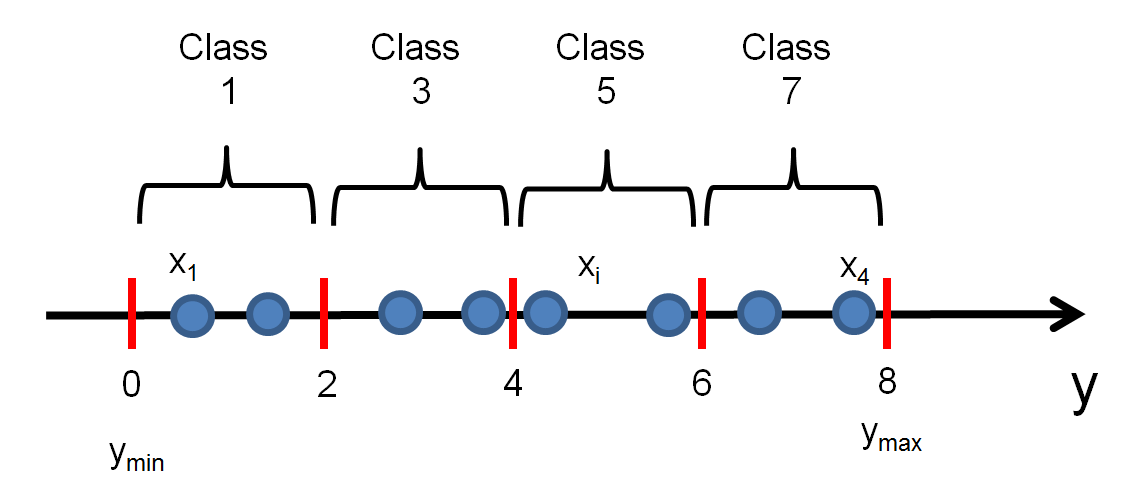
\includegraphics[width=0.5\linewidth]{images/Discretize_binning}
	\caption{Example of discretization by binning a continuous label $y$ into $Q=4$ equal-length intervals. Each interval is associated to a unique class label. In this example, the class label for each interval is equal to the mean in each interval.}
	\label{fig:Discretize_binning}
\end{figure}

\noindent This approach may leads to border effects between the classes. For instance, two samples $\textbf{x}_i$ and $\textbf{x}_j$ that are close to a frontier and that are on different sides of the border will be considered as different, as illustrated in Fig \ref{fig:Discretize_binning_border_effect}. Moreover, a new sample $\textbf{x}_j$ will have its labels $y_j$ assigned to a class and not a real continuous value. 

\begin{figure}[h!]
	\centering
	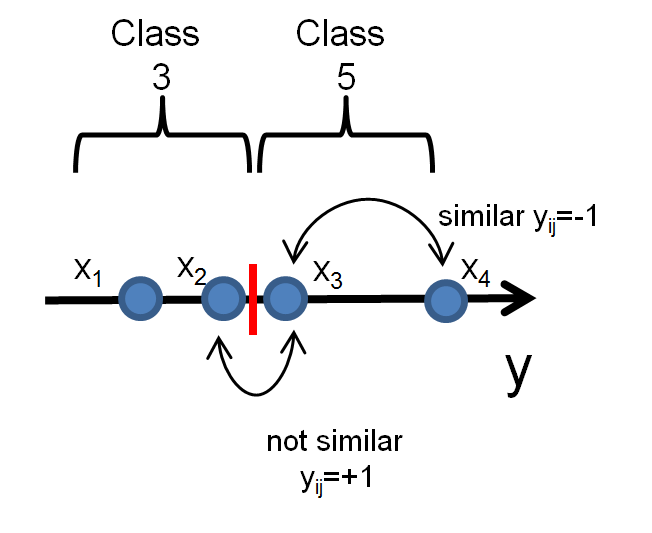
\includegraphics[width=0.4\linewidth]{images/Discretize_binning_border_effect}
	\caption{Border effect problems. In this example, $\textbf{x}_2$ and $\textbf{x}_3$ have closer value labels $y_2$ and $y_3$ than $\textbf{x}_3$ and $\textbf{x}_4$. However, with the discretization $\textbf{x}_2$ and $\textbf{x}_3$ don't belong to the same class and thus are consider as not similar.}
	\label{fig:Discretize_binning_border_effect}
\end{figure}

\noindent The second approach considers the continuous value of $y_i$, computes a $L_1$-norm between the labels $|y_i-y_j|$ and compare this value to a threshold $\epsilon$. Geometrically, a tube of size $\epsilon$ around each value of $y_i$ is built. Two samples $\textbf{x}_i$ and  $\textbf{x}_j$ are considered as similar if the absolute difference between their labels $|y_i-y_j|$ is lower than $\epsilon$ (Fig. \ref{fig:pairwise_label_tube}):
\begin{equation}
y_{ij} = 
\left\{
\begin{split}
\begin{aligned}
-1 & \text{\quad if } |y_i-y_j| \leq \epsilon \\ 
+1 & \text{\quad otherwise }
\end{aligned} 
\end{split}
\right.
\end{equation}

\begin{figure}[h!]
	\centering
	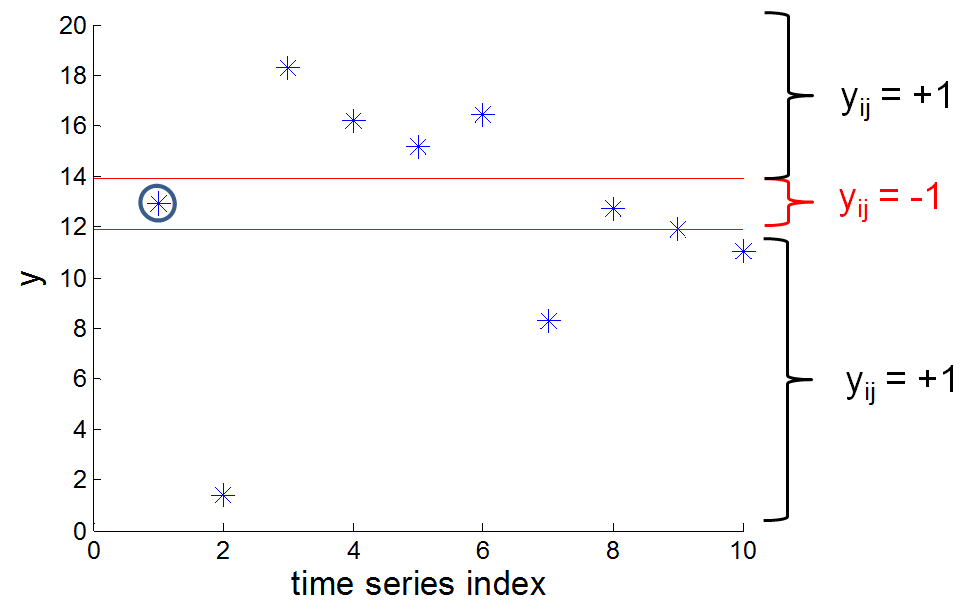
\includegraphics[width=0.65\linewidth]{images/pairwise_label_tube}
	\caption{Example of pairwise label definition using an $\epsilon$-tube (red lines) around the time series $\textbf{x}_i$ (circled in blue). For, time series $\textbf{x}_j$ that falls into the tube, the pairwise label is $y_{ij} = -1$ (similar) and outside of the tube, $y_{ij} = +1$ (not similar).}
	\label{fig:pairwise_label_tube}
\end{figure}

%---------------------------------------------------------------------------
\section{Conclusion of the chapter}
%To learn a multi-modal and multi-scale time series metric for a robust $k$-NN classifier, we detailed in this chapter the different steps of our proposed framework. \\
%First, time series are embedded in the pairwise space using a multi-scale description. Secondly, for each time series, we construct its $m$-nearest neighborhood of the same class and of different classes, forming the pairwise training set. A pairwise {\sc svm} is learnt on the pairwise training set. Finally, the dissimilarity measure is defined to satisfy the required conditions of a metric. 
The adaptation of {\sc svm} in the pairwise space to learn a multi-modal and multi-scale metric $D$ have brought us to propose a pre-processing step before solving the problem such as the neighborhood scaling, and a post-processing step such as defining the metric $D$ as the objective of the {\sc svm} is to separate negative from positive classes.

Choosing a $m$-neighborhood, greater than the $k$-neighborhood, is used in the classifier {\sc svm}. It allows to limit the imposters to invade the neighborhood of the $m$-neighbors while controling the computation complexity.

As we have defined all functions components of our algorithms (learning, testing), we test our proposed algorithms {\sc m}$^2${\sc tml} in the next part on standard datasets of the literature used for classification of univariate time series. 

%%% Local Variables: 
%%% mode: latex
%%% TeX-master: "../roque-phdthesis"
%%% End: 
